%% Spatial-scFormer technical report
%% arXiv submission. Compiles with pdflatex. Figures are vector PDFs in the same directory.
\documentclass[twocolumn,10pt]{article}

\usepackage[a4paper,margin=2.1cm,columnsep=6.5mm]{geometry}
\usepackage[T1]{fontenc}
\usepackage[utf8]{inputenc}
\usepackage{amsmath,amssymb}
\usepackage{graphicx}
\usepackage{booktabs}
\usepackage{siunitx}
\usepackage{xcolor}
\usepackage[colorlinks=true,linkcolor=blue!50!black,citecolor=blue!50!black,urlcolor=blue!50!black]{hyperref}
\usepackage{caption}
\usepackage{framed}
\usepackage{titlesec}
\captionsetup{font=small,labelfont=bf,justification=justified,singlelinecheck=false}
\titlespacing*{\section}{0pt}{2.2ex plus 1ex minus .2ex}{1.2ex plus .2ex}
\titlespacing*{\subsection}{0pt}{1.6ex plus .8ex minus .2ex}{0.8ex plus .2ex}
\setlength{\parskip}{0.3ex}

\graphicspath{{./}}

\setcounter{topnumber}{3}
\setcounter{dbltopnumber}{3}
\setcounter{bottomnumber}{2}
\setcounter{totalnumber}{6}
\renewcommand{\topfraction}{0.95}
\renewcommand{\dbltopfraction}{0.95}
\renewcommand{\bottomfraction}{0.7}
\renewcommand{\textfraction}{0.05}
\renewcommand{\floatpagefraction}{0.72}
\renewcommand{\dblfloatpagefraction}{0.72}
\setlength{\floatsep}{8pt plus 3pt minus 2pt}
\setlength{\textfloatsep}{11pt plus 3pt minus 3pt}
\setlength{\dblfloatsep}{10pt plus 3pt minus 2pt}
\setlength{\dbltextfloatsep}{12pt plus 3pt minus 3pt}
\setlength{\intextsep}{8pt plus 3pt minus 2pt}

\newcommand{\raref}{rare-domain F1}

\begin{document}

\title{\vspace{-2.2em}\bfseries The Lock Is Not the Limit\\[0.3em]
\large What a frozen pseudo-label can and cannot explain about rare-domain detection in spatial transcriptomics}
\author{}
\date{Technical report --- September 2026}
\maketitle

\vspace{-2.5em}

\begin{abstract}
\noindent When a clustering model fails to recover rare tissue domains, the usual suspect is the pseudo-label: frozen, generated by a prior clustering step, and carrying whatever mistakes that step made. The standard remedies are to feed the model spatial structure it was not given, and to let the targets move during training so the model can correct its own initial mistakes. On a human lymph node Visium section (3{,}484 spots $\times$ 18{,}085 genes, 10 annotated domains, 5 rare domains comprising 280 spots, 8.0\% of the section), we tested both remedies against a heterogeneous graph transformer, adding a spot--spot spatial relation in one arm and replacing the frozen Leiden pseudo-label with prototype-based dynamic clustering in another.

Neither recovered the rare domains. The pre-registered primary endpoint, rare-domain F1, did not move in either direction, and we report that outcome as it stands. What the failures explain is more useful than the result. The model trained against the frozen pseudo-label reproduces it almost exactly: at one seed it changed \textbf{0 of 3{,}484} assignments after 100 epochs. The lock is real, and it is what makes the first round of comparisons uninformative, because a model whose output is pinned to its target leaves an architectural component almost no room to change anything. But unlocking it does not help. When we rebuilt the evaluation on an aligned basis (deterministic Top-Z spot--gene graph, gene-wise standardized node inputs, matched tile-and-halo batching) so the output could move freely, the unweighted spatial kNN reduced structural agreement on all three seeds (ARI $-0.118 \pm 0.058$, NMI $-0.141 \pm 0.081$, boundary-F1 $-0.040 \pm 0.014$; all three same-sign with $|\text{mean}| > \text{s.d.}$; only boundary-F1 reaches $p < 0.05$ at $n = 3$). The spatial relation was live, verified by non-zero messages and gradients, and a checkpoint trained on the true graph did not generalize to a degree-matched random graph. Prototype clustering, the remedy meant to correct the initial partition, erased the small cluster it was seeded with.

Two findings transfer beyond this dataset. A rare-domain F1 of zero under a 5-way partition is not a cluster-count limitation: the attainable value over merges of the annotation is 1.0000, and the endpoint is pinned by whether the initial partition happens to contain a cluster below the rarity threshold, which is a property of the partition rather than of the model. And a null result measured under a frozen target is guaranteed by the design, not discovered from the data, a hazard we argue is general rather than specific to this pipeline. We report all negative outcomes alongside the run artifacts, seeds, and protocol hashes needed to verify them.

\vspace{0.6em}
\noindent\textbf{Keywords:} spatial transcriptomics, rare cell detection, negative results, evaluation methodology, pseudo-labeling, graph neural networks
\end{abstract}

\section{Introduction}

Rare cell states and rare tissue domains drive a disproportionate share of the biological questions that motivate spatial assays---the leading edge of a tumor, the immune aggregate that predicts response, the thin structural boundary that separates two tissue compartments. Method papers in this area accordingly present rare-state recovery as a headline capability. The evaluation that would support such a claim is harder than the claim. A rare domain occupies a few percent of a section; the signal that distinguishes it is often one or two markers; and the ground truth itself carries annotation uncertainty at exactly the boundaries that matter.

When a model fails at this, the standard account blames the pseudo-label. The pipeline clusters the data once, freezes that partition as a target, and trains the model to predict it. If the initial clustering merged a rare domain into a larger compartment, the model inherits the mistake and has no way to undo it. Two remedies follow naturally. Give the model spatial structure it was not given, on the argument that tissue geometry carries information expression alone does not. Or stop freezing the target, and let the model correct its own initial clustering as it trains.

We tested both on a human lymph node section. The answer was no to each, and the reason the answer was no is more useful than the remedies. This report is about that reason. It is not a method paper, and it does not end with a better detector. It is an account of what had to be true for the question to be answerable at all, and of what the negative result reveals about where the failure actually lives.

We report the negative outcome with full instrumentation because negative results in this area are under-represented in the literature, and their absence distorts it. When only positive outcomes are written up, the apparent success rate of architectural modifications is inflated, and the diagnostics that explain why a modification fails are lost. The artifacts required to falsify our conclusions, including per-seed metrics, protocol hashes, construction proofs, and null controls, are all preserved. Section~\ref{sec:repro} states exactly where each number comes from.

\section{Setup}
\label{sec:setup}

\subsection{Data}

One human lymph node section (10x Genomics Visium~\cite{stahl,rao}), 3{,}484 spots $\times$ 18{,}085 genes, with 10 annotated tissue domains. Five domains are rare under the standard $\leq 5\%$ criterion: follicle (96 spots), medulla vessels (80), subcapsular sinus (73), hilum (23), and trabeculae (8), totaling 280 spots or 8.0\% of the section.

These are not compact regions, and their shape is central to why the task is hard. As Figure~\ref{fig:f1} shows, they form a thin ring-like structure (follicle), narrow bands inside the medulla (medulla vessels), and a handful of isolated points (hilum, trabeculae). A coarse partition---one with, say, five clusters---tends to absorb such structures into the larger compartment they border. This is not a hypothetical failure mode; it is the observed behavior of the default pipeline, and Section~\ref{sec:construction} proves that it is not fixable by changing the number of clusters.

\begin{figure*}[tbp]
\centering

\includegraphics[width=\textwidth]{fig1_ground_truth_rare_domains}
\caption{The rare domains and why they are hard. Ground-truth annotation with the five rare domains pulled out. They occupy 8.0\% of the section and are shaped as a thin capsule ring (follicle, 2.76\%), narrow medullary bands (medulla vessels, 2.30\%), and isolated points (hilum, 0.66\%; trabeculae, 0.23\%). A bar chart of domain shares (panel c) conveys the imbalance but not the geometry, and the geometry is what makes the rare-domain F1 endpoint non-trivial. Spot geometry is restored from Visium array coordinates (100\,\textmu m column pitch, 86.6\,\textmu m row pitch); each tile is the spot's Voronoi cell.}
\label{fig:f1}
\end{figure*}

\subsection{Endpoints}

Our primary endpoint is rare-domain F1: micro-averaged F1 over the five rare domains, treating a predicted cluster as a rare-domain prediction if it occupies less than 4.5\% of the section, a cutoff set slightly below the $\leq 5\%$ convention to keep the criterion strict (Section~\ref{sec:markers}). We report the adjusted Rand index (ARI)~\cite{hubert,sklearn} and normalized mutual information (NMI) against the annotated domains as secondary endpoints. Both measure agreement between two partitions of the same spots, ARI corrected for chance and NMI as shared information normalized to $[0,1]$; a value near zero means the partition carries essentially no information about the annotation. As a structural endpoint we also report boundary-F1, which scores how well the boundaries a partition draws between clusters coincide with the true domain boundaries, and is sensitive to a partition that places the right clusters in the wrong places.

Two properties of this endpoint govern its interpretation, and both are easy to get wrong. An absolute rare-F1 value means nothing on its own, because a partition carries an attainable rare-F1 of its own, the value it reaches before any model is trained. That value is the reference a model has to beat. Reporting rare-F1 $= 0.39$ on a partition whose own rare-F1 is already $0.39$ describes a model that added nothing, even though the number looks favourable. The second property concerns what a small cluster demonstrates. A predicted cluster falling below the threshold is not evidence of rare-domain detection: if rare spots make up 8.0\% of the section and a small cluster contains 6\% rare spots, that cluster is depleted in rare spots rather than enriched. We therefore test enrichment against the section-wide base rate before treating a small cluster as a rare domain.

\subsection{Model and training}

The backbone is a heterogeneous graph transformer over spot and gene nodes (104 hidden dimensions, 8 heads, 3 layers), trained for 100 epochs with a KL reconstruction objective, following the scFormer architecture~\cite{scformer}. Two variables are under test, and it is worth stating them in plain terms before the technical description. The first asks whether telling the model which spots are physical neighbours in the tissue helps it define domains, beyond what expression alone provides. The second asks whether letting the cluster targets move during training helps the model recover domains that its initial clustering would otherwise merge into a larger one.

Described precisely, the first variable is whether a spot--spot spatial relation enters message passing as a third relation type, using $k$-nearest neighbours on the spatial coordinates. In this first version the graph is unweighted and no auxiliary spatial loss is added, so any effect can be attributed to the relation itself rather than to a new loss term. The construction follows the first stage of the SpaMICS reference design~\cite{spamics}, which builds a spot graph and then refines it; we implement only the unweighted construction. The second variable is whether the clustering head predicts a frozen Leiden pseudo-label~\cite{traag} through a linear layer, or instead maintains a set of prototype vectors, one per cluster, that are recomputed during training. A spot is assigned to the prototype it is most similar to, and only spots whose assignment confidence exceeds a threshold contribute to the prototype update, so that ambiguous spots are left uncommitted rather than forced toward a cluster. This follows the DEC~\cite{dec} and DESC~\cite{desc} family. We deliberately exclude variable $K$ and split--merge~\cite{deepdpm}, so that only the fixed-versus-dynamic label question is under test.

Figure~\ref{fig:f9} places these two variables against the design space and marks which arms were actually executed. Not every cell of the matrix was run: the project was stopped under its registered gate after the aligned-basis comparison failed its criterion (Section~\ref{sec:aligned}), so the full four-arm ablation, the $\tau/\delta$ calibration, and graph refinement were not executed. We make no claims about them. One qualification on the registration, since it bears on how the gate should be read: the protocol was registered before the aligned-basis runs but after the first two baseline runs had begun, and it covers the aligned-basis comparison specifically rather than the study as a whole. The analyses in Sections~\ref{sec:headroom} and~\ref{sec:construction} were not part of it.

\begin{figure*}[tbp]
\centering
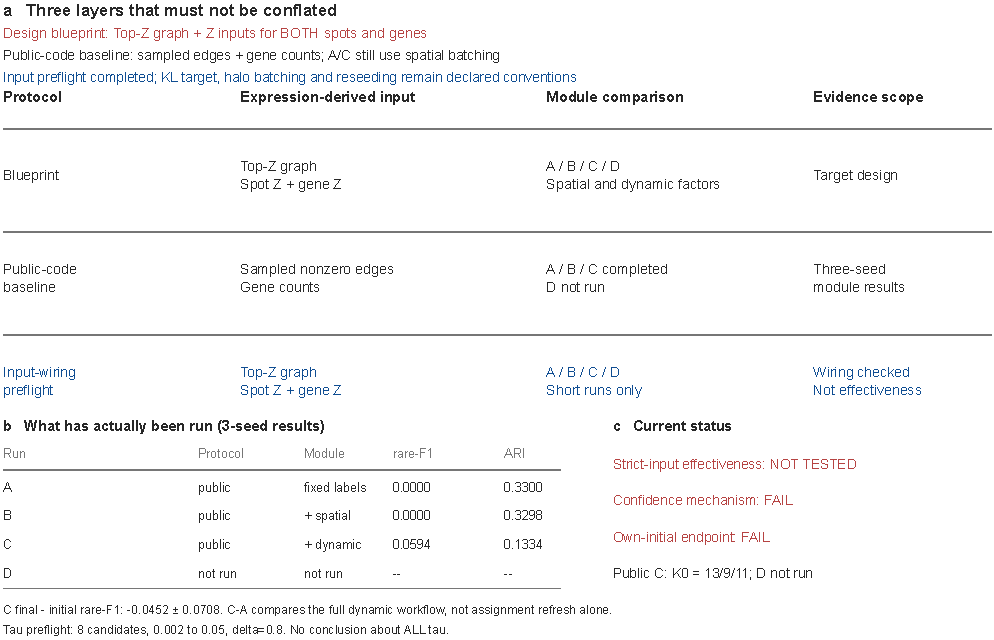
\includegraphics[width=\textwidth]{fig9_method_design}
\caption{The design space and what was actually run. Method schematic against the ablation matrix, marking which arms were executed and on which input basis. The two manipulated variables are the presence of a spot--spot spatial relation and the choice between a frozen pseudo-label head and prototype-based dynamic clustering. The public-code basis refers to the upstream implementation's sampled edge construction and raw-count inputs; the aligned basis refers to the deterministic Top-Z graph with standardized node inputs.}
\label{fig:f9}
\end{figure*}

\subsection{What ``measurable'' requires}

Before comparing two arms we require that the model be able to deviate from its starting point at all. We quantify this directly: align the final assignments to the pseudo-label by Hungarian matching and count how many of the 3{,}484 spots changed. This ``headroom'' number is the ceiling on any effect the comparison could possibly detect, and as Section~\ref{sec:headroom} shows, it is small enough to invalidate the comparison it was meant to support.

This diagnostic is trivial to compute and, to our knowledge, is not standard practice. We suggest it should be.

\section{Results}
\label{sec:results}

\subsection{The frozen target leaves almost no room to measure anything}
\label{sec:headroom}

The model trained against a frozen Leiden pseudo-label reproduces that label. Under the default settings, the agreement between prediction and pseudo-label reaches ARI 1.0000, 0.9972, and 0.9741 across the three seeds (seeds 1, 42, 0), corresponding to \textbf{0, 4, and 38} changed assignments out of 3{,}484---at one seed, none at all.

That number defines the ceiling. When we compared the spatial-relation arm against the expression-only arm on an initial partition that \emph{does} contain a rare cluster, the spatial arm deviated from the pseudo-label by \textbf{7, 0, and 5} spots, against 0, 1, and 65 for the baseline arm; the between-arm gaps were 7, 1, and 69 spots. The larger deviation came from the \emph{baseline} arm drifting, not from the spatial arm improving. Which arm deviates, and by how much, is determined by the seed rather than by the relation.

This makes the comparison uninterpretable, and the reason is structural. The paired difference in rare-F1 across the three seeds was $-0.0042$, $0.0000$, and $+0.0085$---sign-inconsistent, with a mean ($+0.0014$) smaller than the standard deviation of the baseline arm's own seed-to-seed spread ($0.0068$). An effect of the size we were looking for cannot be distinguished from the sampling noise of the baseline in this regime, regardless of how many seeds we run.

The mechanism is worth stating precisely, because it is not specific to this dataset. A model whose training signal is a frozen clustering and whose capacity is sufficient to fit it will converge to that clustering. Once it does, its output is a function of the initial partition, and any architectural component, whether a spatial relation, an attention variant, or a loss term, acts on a quantity that is already determined. The component can perturb which few spots flip; it cannot change the partition. Twenty seeds of this would measure the perturbative noise more precisely and would not approach the question.

\begin{figure*}[tbp]
\centering
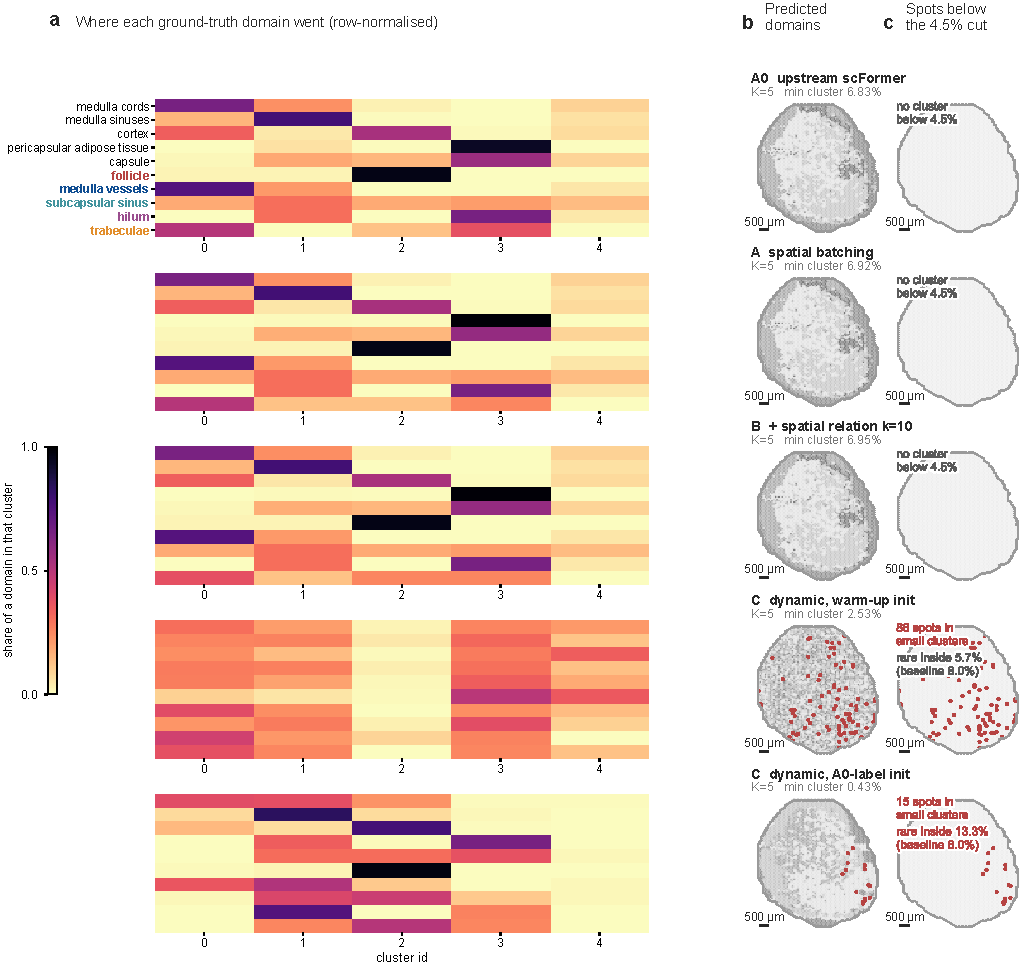
\includegraphics[width=\textwidth]{fig2_per_arm_partitions}
\caption{Per-arm spatial partitions. Predicted partitions for the baseline and spatial arms alongside the contingency structure against the ground truth, showing where rare spots are assigned. On the default partition no arm produces a sub-threshold cluster, which is why the rare-domain F1 endpoint cannot move in that regime: the limitation is the partition, not the comparison. Spot geometry is restored from Visium array coordinates as in Figure~\ref{fig:f1}.}
\label{fig:f2}
\end{figure*}

\begin{framed}
\noindent\textbf{The central methodological finding.} A frozen pseudo-label that the network nearly reproduces converts architectural comparison into a measurement of noise. The correct response is not more seeds; it is to change the regime so that the output is no longer pinned.
\end{framed}

\subsection{\texorpdfstring{Rare-domain F1 $=0$ is not a cluster-count artifact}{Rare-domain F1 = 0 is not a cluster-count artifact}}
\label{sec:construction}

A natural explanation for failing to recover rare domains is that the partition simply has too few clusters to place them. Under a 5-way partition, the five rare domains (8.0\% of the section) have nowhere to go.

This explanation is false as stated, and we can show why by construction. We exhaustively enumerated all 42{,}525 ways of merging the 10 annotated domains into exactly 5 groups. The maximum attainable rare-F1 is \textbf{1.0000}. Three clusters suffice: one containing follicle $+$ hilum $+$ trabeculae (127 spots, 3.65\%), one containing medulla vessels $+$ subcapsular sinus (153 spots, 4.39\%), and one containing the remaining 3{,}204 spots, which the 5-way enumeration accommodates by subdividing that remainder. Both small clusters are 100\% rare. What this establishes is precise and narrower than it may first appear: $K = 5$ is not a hard ceiling on attainable rare-F1. The construction merges ground-truth annotated domains, an operation no unsupervised pipeline has access to, so it bounds what is \emph{achievable}, not what an unsupervised partition will find.

The real constraint is upstream. The default Leiden resolution on the expression space (0.5) does not produce small clusters at all---its minimum cluster occupies 6.89\% of the section, above the threshold, so rare-F1 is pinned at zero by construction. Sweeping the resolution changes this directly: at resolution 0.2 the partition yields a 96-spot cluster that is 75.0\% rare (rare-F1 $0.3830$), and at resolution 0.8 a 102-spot cluster that is 73.5\% rare (rare-F1 $0.3927$). Both are properties of the \emph{initial partition}, present before any model runs.

As Figure~\ref{fig:f8} shows, this is a frontier rather than a monotone improvement: the resolutions that produce small clusters (0.2, 0.8) are not the ones that maximize ARI (0.3). The two endpoints are not aligned on this dataset, which is itself a useful fact for anyone tuning an initial partition.

\begin{figure*}[tbp]
\centering
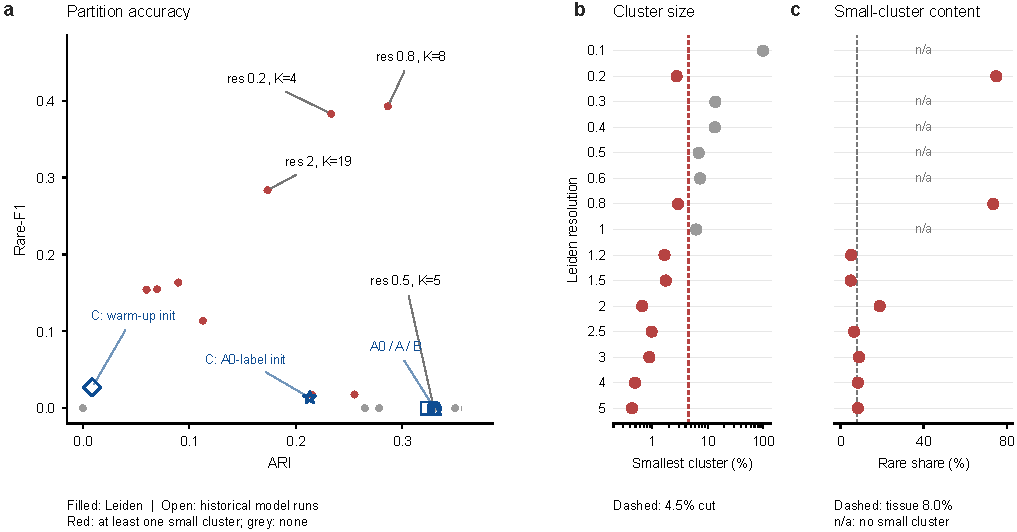
\includegraphics[width=\textwidth]{fig8_baseline_frontier}
\caption{The initial-partition frontier. Rare-domain F1 and ARI across Leiden resolutions. The endpoint is not monotone in resolution: the resolutions that produce a sub-threshold cluster (0.2, 0.8) are not the ones that maximize ARI (0.3). Panels show the minimum cluster share and the rare share within the smallest cluster, with the 4.5\% prediction threshold and the 8.0\% section-wide rare base rate drawn as reference lines; resolutions producing no small cluster are marked n/a. Both panels are properties of the partition alone, computed before any model runs.}
\label{fig:f8}
\end{figure*}

One caveat belongs with this result. The 0.3927 attained at resolution 0.8 comes entirely from the follicle domain: 74 of the 102 rare spots in the cluster are follicle (recall 0.771), while medulla vessels, hilum, and trabeculae have recall 0 and subcapsular sinus captures a single spot. Recovery of \emph{one} rare domain is not recovery of rare domains, and we report it as the former.

The practical consequence is a rule that requires no ground truth to apply: \emph{an initial partition must contain at least one cluster below the rarity threshold, or the rare-domain endpoint is pinned at zero by construction.} On this dataset, resolution 0.5 fails that test and resolutions 0.2 and 0.8 pass it. This is checkable before training, and it would have saved us the first round of experiments.

\subsection{Spatial edges must survive batching before the relation can be tested}
\label{sec:batching}

An architectural change can only be evaluated if it is actually active during training. For a spatial relation this is not automatic, because the upstream batching samples spots uniformly, scattering a batch of 30 spots across the entire section. Under that scheme only \textbf{0.78\%} of spatial edges have both endpoints inside the same batch. The relation is present in the graph and almost never exercised in message passing.

Replacing uniform sampling with spatial median bisection raises in-batch retention to 69.4\%, and adding a one-hop halo brings it to \textbf{100\%} at the cost of growing an effective batch from 30 spots to 58--81. Only after this change is a spatial-arm comparison a test of the spatial relation rather than a test of the sampler.

\begin{figure*}[tbp]
\centering
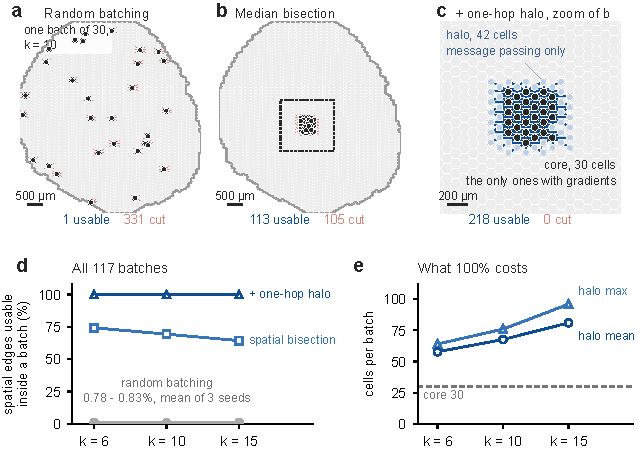
\includegraphics[width=\textwidth]{fig5_edge_retention}
\caption{Spatial edges must survive batching to be testable. (a) The upstream uniform sampler scatters a batch's 30 spots across the whole section, breaking almost every spatial edge. (b) Spatial median bisection makes a batch a contiguous tissue block, retaining most edges. (c) A one-hop halo recovers the remainder. (d) Global in-batch retention across $k=6/10/15$: $0.78\% \rightarrow 64\text{--}74\% \rightarrow 100\%$. (e) The cost: the effective batch grows from 30 spots to 58--81. Without this step, an arm comparison measures the sampler rather than the relation.}
\label{fig:f5}
\end{figure*}

This point generalizes past spatial relations. Any modification that acts over a graph structure, whether spatial adjacency, gene--gene edges, or higher-order relations, is subject to the same failure: if the batching scheme destroys the structure the modification depends on, the experiment measures the batching. We found it worth checking explicitly, and the check is cheap: count how many edges of the new relation type have both endpoints in the same batch.

\subsection{On an aligned basis, unweighted spatial kNN degrades structure}
\label{sec:aligned}

Having established that the fixed-target regime cannot resolve the comparison, we rebuilt the evaluation on a basis where it can. The aligned basis uses a deterministic Top-Z spot--gene graph, selecting edges by $Z$-score rank rather than by stochastic sampling, standardizes the gene-node inputs, and applies the tile-and-halo batching of Section~\ref{sec:batching} identically to both arms. Both arms share an identical initial model state, and the only difference between them is whether the unweighted spatial kNN relation, at $k = 10$, is enabled. We ran three seeds for 30 epochs with a KL-only objective, so that no clustering term confounds the representation comparison.

It is worth showing that the rebuild achieved what it was for rather than asserting it. The test is the same headroom measurement as in Section~\ref{sec:headroom}: how far the output sits from the pseudo-label. Under the aligned basis, clustering the resulting embedding differs from the Leiden pseudo-label on 62\%, 51\%, and 60\% of the 3{,}484 spots across the three seeds, against 0\%, 0.03\%, and 1.9\% in Section~\ref{sec:headroom}. The output is no longer pinned, which is the property the comparison needed.

That said, the rebuilt comparison is not the same experiment made measurable. It drops the clustering objective in favour of a reconstruction-only objective and reports representation metrics at 30 epochs, so it answers a question about representation structure rather than one about rare-domain recovery under clustering. We treat the two as separate measurements and draw no single conclusion across them.

Under this basis the comparison becomes measurable, and it is negative. Table~\ref{tab:p2} reports the paired differences. Enabling the spatial relation changes ARI by $-0.118 \pm 0.058$, NMI by $-0.141 \pm 0.081$, and boundary-F1 by $-0.040 \pm 0.014$. All three are same-sign across all three seeds, and for all three the absolute mean exceeds the standard deviation. That last criterion was pre-registered, and it is a decision rule rather than a significance test: with $n = 3$ it is equivalent to $|t| \approx 1.73$, or $p \approx 0.22$. Reporting the paired tests explicitly, only boundary-F1 reaches $p < 0.05$ uncorrected ($p = 0.039$); ARI ($p = 0.073$) and NMI ($p = 0.094$) do not. The effects are large and consistent in direction, but the establishment is limited by the seed count, and we state it that way rather than as an established result.

Two further outcomes belong in the same table. kNN label purity improves, by $+0.0079 \pm 0.0063$, and it satisfies the same same-sign and $|\text{mean}| > \text{s.d.}$ rule in the favourable direction, so this is not a case of every reported quantity moving one way. The registered gate nonetheless failed, because it required improvement on the primary endpoint (rare-domain F1) and on ARI, and neither was met. Rare-F1 is directionless ($+0.059 \pm 0.099$, $p = 0.41$), with one seed contributing the entire spread, and we note that the primary endpoint of the study therefore did not move negatively, it failed to move at all.

\begin{table*}[tbp]
\centering
\caption{Aligned-basis paired comparison (B0 $-$ A$^\ast$), three seeds. Same-sign means all three per-seed differences share a sign. The last column is the two-sided paired $t$-test on $n=3$. Three metrics are negative on every seed with $|\text{mean}| > \text{s.d.}$, but with $n=3$ that decision rule is equivalent to $|t| \approx 1.73$ ($p \approx 0.22$) and is a pre-registered criterion rather than a significance test; only boundary-F1 reaches $p < 0.05$ uncorrected. The kNN-purity difference satisfies the same decision rule in the favourable direction. The rare-F1 difference is carried by one seed and is not interpretable.}
\label{tab:p2}
\small
\begin{tabular}{lS[table-format=-1.4]S[table-format=1.4]lccc}
\toprule
Metric & {Mean} & {s.d.} & {Per-seed values} & {Same sign} & {$|\text{mean}|>\text{s.d.}$} & {$p$ ($n{=}3$)} \\
\midrule
ARI          & -0.1177 & 0.0585 & $-0.145/-0.051/-0.158$ & yes (neg.) & yes & 0.073 \\
NMI          & -0.1411 & 0.0806 & $-0.171/-0.050/-0.203$ & yes (neg.) & yes & 0.094 \\
boundary-F1  & -0.0399 & 0.0141 & $-0.047/-0.024/-0.049$ & yes (neg.) & yes & 0.039 \\
rare-domain F1 & 0.0592 & 0.0986 & $+0.173/0.000/+0.005$ & no & no & 0.407 \\
kNN purity   & 0.0079 & 0.0063 & $+0.015/+0.002/+0.007$ & yes (pos.) & yes & 0.162 \\
\bottomrule
\end{tabular}
\end{table*}

\begin{figure*}[tbp]
\centering
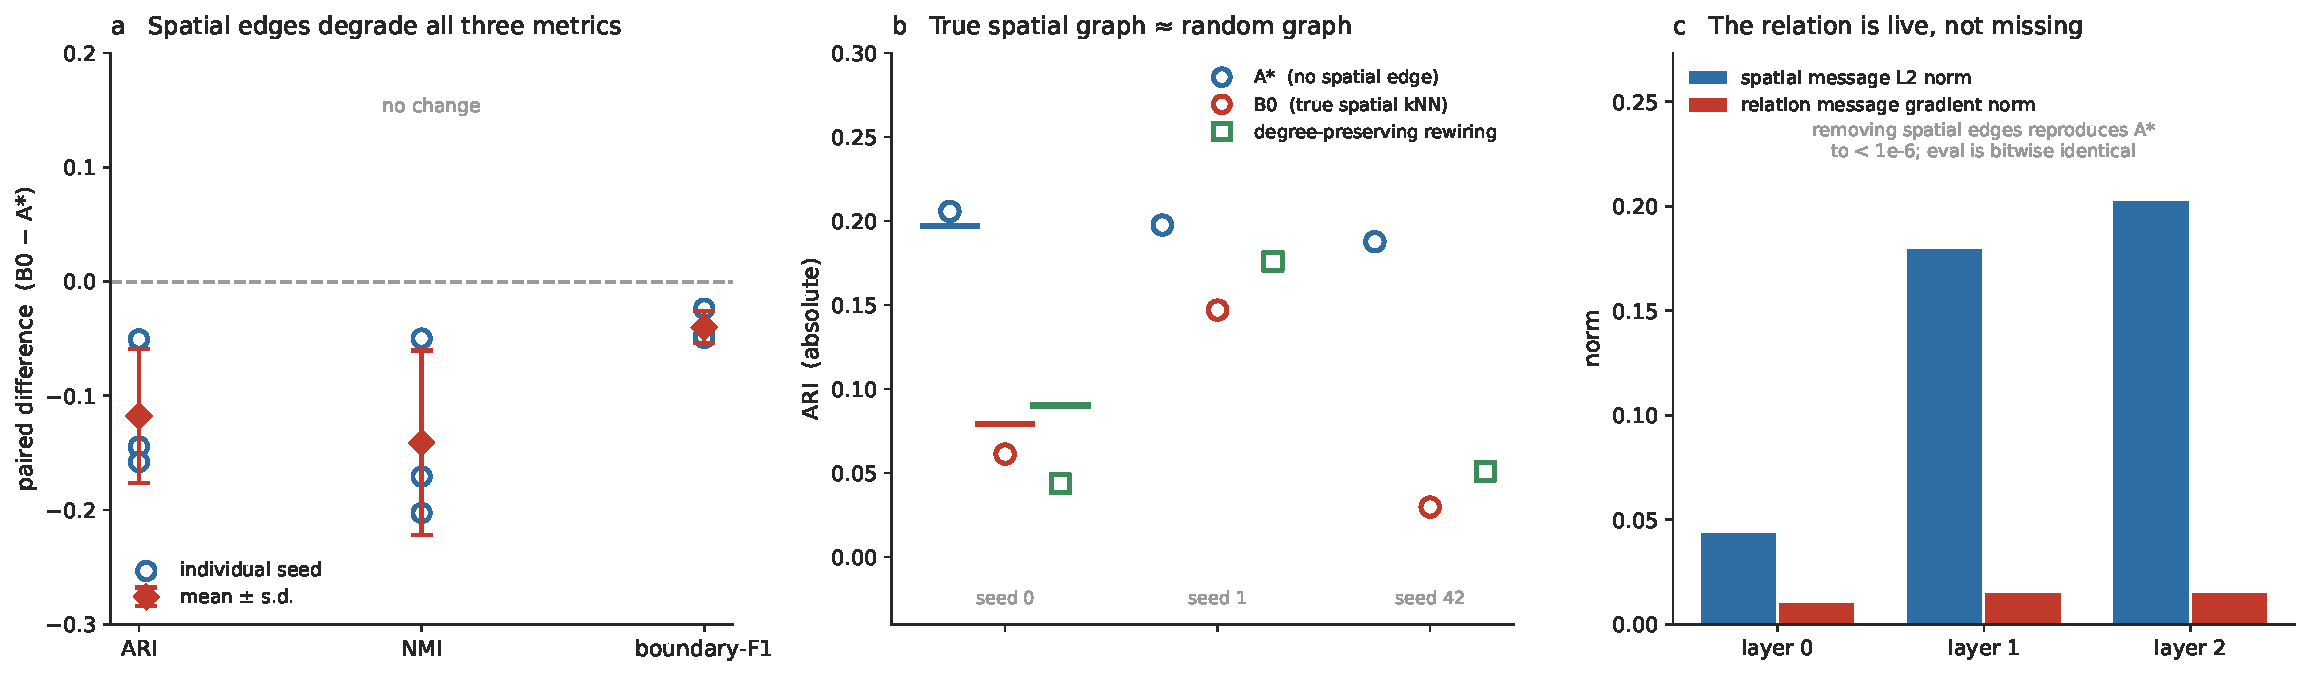
\includegraphics[width=\textwidth]{fig12_p2_core_result}
\caption{The aligned-basis result and its null controls. (a) Paired differences B0 $-$ A$^\ast$ for the three structural metrics; all three lie left of the no-change line with the mean beyond one standard deviation. (b) Absolute ARI by arm: the true spatial graph (B0) performs no better than a degree-preserving random rewiring of itself, which places the effect in the added edge set's presence rather than its spatial topology. (c) Wiring evidence---spatial message norms and relation-message gradient norms are non-zero at every layer, so the degradation is not a missing connection.}
\label{fig:f12}
\end{figure*}

The degradation is not explained by the relation failing to reach the model. Spatial messages are non-zero at all three layers, the relation's message gradients are non-zero, disabling the spatial edges reproduces the baseline arm's output to within $10^{-6}$, and repeated evaluation is bitwise identical. The spatial relation is consumed by the model, and consuming it makes structural agreement worse.

Two controls probe whether the spatial topology is doing any work, and both must be read with an important caveat. Each replaces the spatial edges at inference time on the checkpoint trained with the true graph, rather than retraining the model on the modified graph. The project's own protocol labels these ``diagnostic necessity evidence only, not retrained causal null'', and we adopt that scope. Such a control tests whether a trained model generalizes to a different graph; it does not establish what the model would learn if trained on one.

With that caveat, the results are these. Permuting the coordinates, which destroys spatial meaning while preserving the pipeline, yields ARI $0.016$, $0.134$, and $0.080$ across the three seeds. Replacing the spatial graph with a random graph of identical degree sequence yields ARI $0.044$, $0.176$, and $0.051$, against $0.061$, $0.147$, and $0.030$ for the true spatial graph. The two are not distinguishable in the mean, and on two of the three seeds the rewired graph scores slightly higher; the per-seed values of the rewiring control span $0.044$ to $0.176$ against a true-graph span of $0.030$ to $0.147$. The honest reading is that at this seed count the trained checkpoint does not visibly transfer to a degree-matched random graph.

This is a parity result, and we state it at that strength. It does not license the stronger claim that the pipeline fails to extract spatial topology, which would require retraining on the rewired graph for all three seeds, or an equivalence test with a stated margin. Both remain open. One further observation cuts across the framing: both the true spatial graph and its rewiring fall well below the relation-free baseline, so the dominant effect in this comparison is that adding an unweighted third relation type perturbs the representation at all. That is a broader and less spatial-specific claim than one about topology, and it suggests the degradation may be driven by the presence of an extra relation rather than by its spatial content. A control that could separate these, such as a non-spatial relation of matched edge count, was not run.

A third control separates a different effect, and its interpretation needs care. Disabling the spatial message while leaving the sampler and graph construction intact returns ARI to $0.237$, $0.207$, and $0.208$, above the relation-free baseline on all three seeds. Because both the baseline and this control use the same tile-and-halo sampler and differ only in whether the third relation was present during training, the difference is most naturally read as a residual training-time effect of the spatial relation rather than as a sampling artifact. We report it as an observation that does not fit the simple story, and we do not have a control that isolates its cause.

The result is bounded, and the boundary matters. It falsifies unweighted spatial kNN at $k=10$, as implemented here, on this dataset, under this basis. It does not establish that spatial relations are unhelpful in general. The positive spatial results cited here weight or refine the graph, using expression to gate or reweight spatial edges rather than treating them as uniform, as in STAGATE~\cite{stagate}, GraphST~\cite{graphst}, and SpatialGlue~\cite{spatialglue}, and in gene--gene relation construction of the kind used by stKeep~\cite{stkeep}. A single negative configuration cannot adjudicate that design space. One observation cuts across the framing: both the true spatial graph and its degree-matched rewiring fall well below the relation-free baseline, so the dominant effect here is that adding an unweighted third relation type perturbs the representation, which is a narrower claim than one about spatial topology specifically. The natural next question, which our gate stopped us from pursuing, is whether a \emph{weighted} spatial graph would separate from the degree-matched control.

One caveat on the numbers: these are 30-epoch warm-up representation metrics. The baseline arm sits at ARI $\approx 0.21$ and boundary-F1 $\approx 0.60$ here, and these values should not be compared with the 100-epoch figures reported elsewhere in this report. That choice of basis is deliberate, since 30 epochs is where the target no longer pins the output, but it also means the sign is measured before the representation has converged, and we have not tested whether it persists at 100 epochs.

\subsection{Prototype clustering erases the small cluster it is given}
\label{sec:prototype}

The second prescription, replacing the frozen pseudo-label with prototypes updated during training, produces a parallel failure. Its premise is that the model can correct an initial partition that has merged rare domains into a larger one.

That premise does not hold on this data. The warm-up representation under the public-code basis, trained for 30 epochs with a KL-only objective, carries almost no domain structure: ARI $0.0006$ against the annotation, kNN label purity $0.2331$ against a chance level of $0.2205$, and an effective rank of $22.35$. The representation is high-dimensional but the signal is absent rather than collapsed---it is not that the embedding degenerated to a point, but that it spread out in directions unrelated to domain identity. For comparison, the expression space that generates the pseudo-labels attains ARI $0.3308$ and kNN purity $0.6009$ on the same data. Prototypes initialized on the former are initialized on noise.

The input basis matters here, and the two warm-up comparisons in this report differ because of it. The aligned basis of Section~\ref{sec:aligned} yields a considerably stronger 30-epoch representation (ARI $\approx 0.21$) than the public-code basis probed above (ARI $0.0006$), because it uses the deterministic Top-Z graph and standardized node inputs. The prototype results in this section come from the public-code basis, and we did not re-run the prototype arm on the aligned basis, so the diagnosis below is scoped to the former.

\begin{figure*}[tbp]
\centering
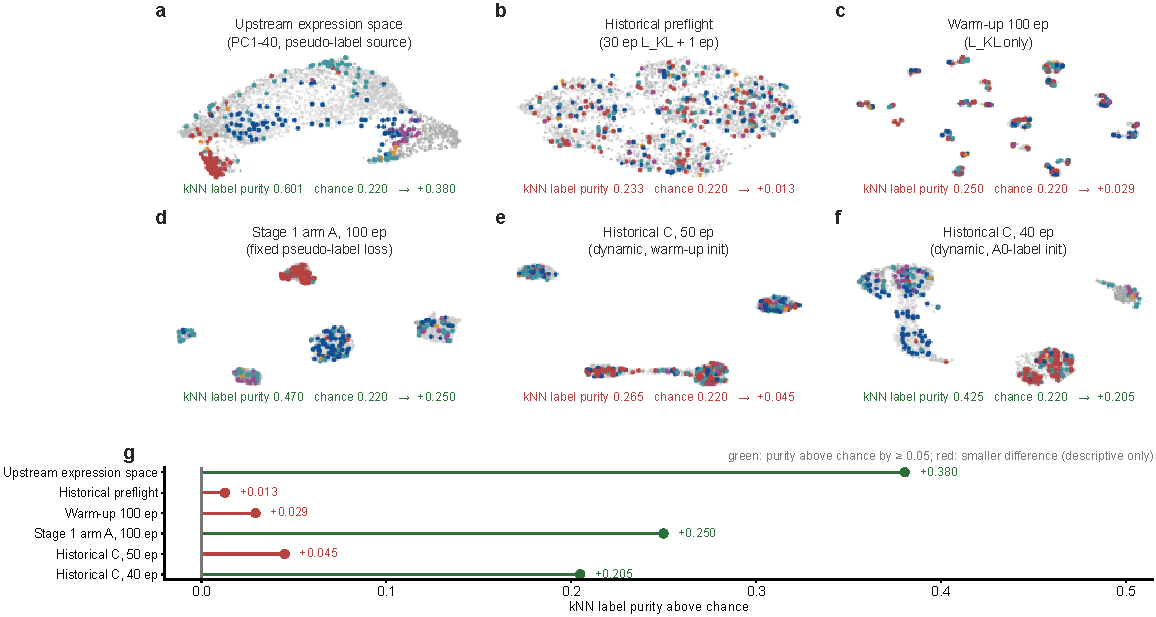
\includegraphics[width=\textwidth]{fig6_representation}
\caption{What the warm-up representation contains, under the public-code basis. Embedding projections and kNN label purity for the representations involved, against the expression space that generates the pseudo-labels. The 30-epoch KL-only warm-up sits near the chance level of 0.2205, while the pseudo-label source space reaches 0.6009; the panels also show longer warm-up runs and the historical dynamic-clustering variants they were compared against. This is the candidate bottleneck that makes prototype initialization unreliable, reported as a candidate explanation rather than a proven unique root cause. Note that the aligned basis of Section~\ref{sec:aligned} produces a stronger warm-up representation than the one shown here.}
\label{fig:f6}
\end{figure*}

When we instead seed the prototypes with a partition that \emph{does} contain a rare cluster (resolution 0.8, rare-F1 $0.3927$), the update erases it. At a refresh interval of 5 epochs, rare-F1 falls from $0.3927$ to $0.0619$, and the original cluster fragments into six pieces containing 302 spots of which 18 are rare---5.96\%, \emph{below} the section-wide 8.0\% base rate. This is fragmentation, not enrichment: the rare spots are scattered into small clusters that are rarer-depleted on average than the section as a whole.

Extending the refresh interval to 30 epochs repairs the geometry. First-refresh churn, the fraction of spots whose assignment changes at the first refresh, falls to 37.6\%, 24.5\%, and 37.0\% across seeds, and prototype cosine maxima to 0.47--0.72, against near-collinear values above 0.92 under the shorter interval. ARI then recovers to 0.228--0.272. But the rare-domain endpoint does not follow: rare-F1 remains $0.0558$, $0.0069$, and $0.0182$, with absolute rare counts of 11, 1, and 3 spots. Adjusting the prototype loss weight downward lowers ARI further and drives rare-F1 to zero.

\begin{figure*}[tbp]
\centering
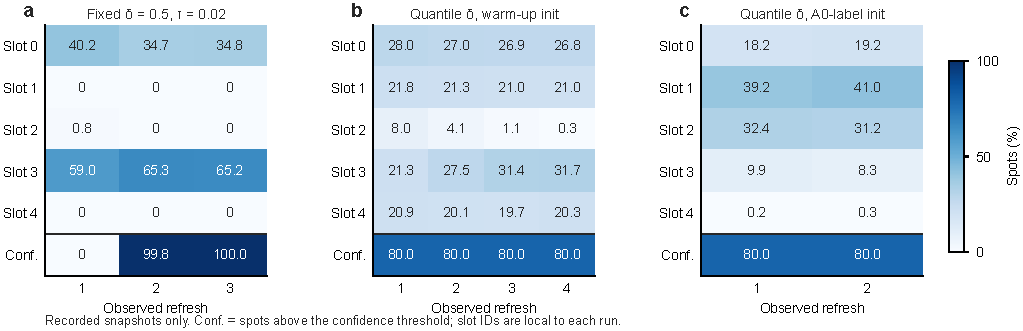
\includegraphics[width=\textwidth]{fig7_refresh_trace}
\caption{Prototype refresh dynamics. Cluster-slot occupancy and confident-fraction trajectories through a refresh cycle, for the historical dynamic-clustering variants. Each row is one cluster slot; the bars show how many spots each slot holds after a refresh, and the confidence trace shows what fraction of spots clear the confidence threshold. The geometry can be repaired by lengthening the refresh interval (fewer active slots collapse, prototypes become less collinear), and ARI recovers---but the rare-domain endpoint does not. Adjusting the loss weight changes how early training stalls without restoring the small cluster.}
\label{fig:f7}
\end{figure*}

\begin{figure*}[tbp]
\centering
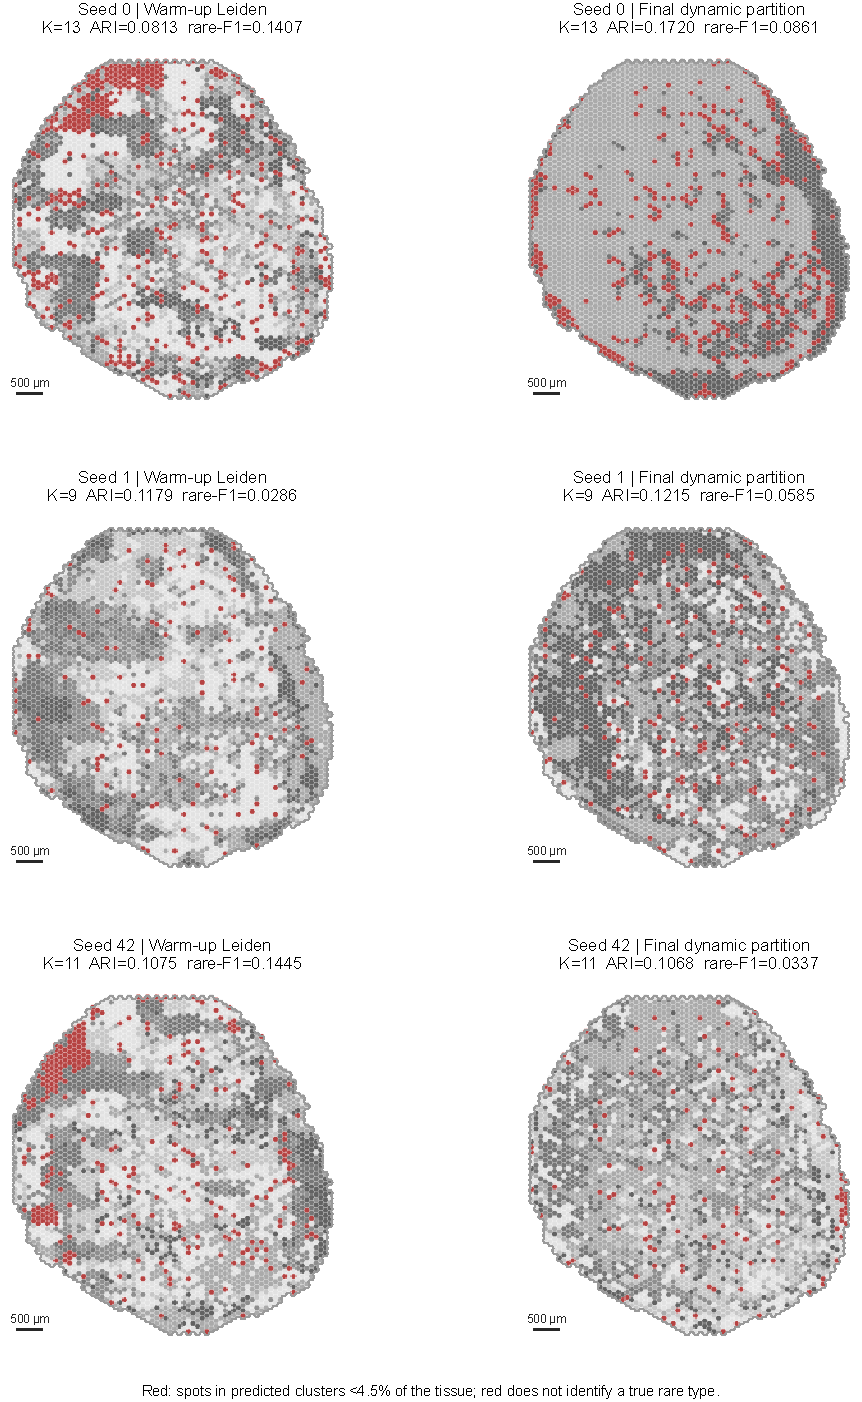
\includegraphics[width=0.72\textwidth]{fig11_c_init_final}
\caption{The small cluster is dissolved, not relabeled. Initial versus final spatial partitions for the dynamic-clustering arm (arm C), one panel per seed, under the public-code basis. These are a different configuration from the single-seed result quoted in the text ($0.3927 \rightarrow 0.0619$, which ran on the partition seeded from resolution 0.8), so the per-seed rare-F1 values differ; what both show is the same behavior. The initial cluster is gone in the final assignment, and the residual small clusters are reseeded or collapsed slots rather than the original rare niche. Red marks predicted clusters occupying less than 4.5\% of the section, which is not the same as a true rare domain, and cluster indices are not comparable across panels. Spot geometry is restored from Visium array coordinates as in Figure~\ref{fig:f1}.}
\label{fig:f11}
\end{figure*}

We report this as a scoped negative, with the scope stated precisely. The refresh interval was swept across all three seeds; the prototype loss weight was probed at seed 0 only, so the loss-weight observation below rests on a single run. The refresh interval governs geometric health and ARI; the loss weight governs how early training stalls. Neither restores the small cluster. What neither does, on the evidence we have, is preserve a small cluster through a prototype update on a representation this weak. The mechanism, as far as we can tell from the refresh traces, is that the prototype update is computed on a representation where domain structure is near-chance, so the high-confidence spots that dominate the update are not the ones that define the rare niche.

\subsection{Where the rare signal actually lives}
\label{sec:markers}

One biological boundary constrains how any of the above should be read. Applying a Wilcoxon test to each annotated rare domain (adjusted $p < 0.05$, in-domain detection $\geq 60\%$, fold-change $\geq 2$, scanned over the full ranking rather than a truncated candidate pool), only \textbf{follicle} has an unambiguous, spatially specific marker: CXCL13, detected in 89.6\% of the domain, expressed at 10.1$\times$ the section mean, with 45 of the 96 top-expressing spots inside the domain (17$\times$ random enrichment).

Hilum has a statistically significant gene (COL1A2) that is \emph{not} spatially specific---collagen is high across the entire capsule, so only 2 of the 23 top-expressing spots fall inside hilum. It passes the statistical criteria without the expression field localizing the domain. The remaining three domains satisfy no gene at all: their best candidates reach fold-changes of 1.9 (medulla vessels), in-domain detection of 48\% (subcapsular sinus), and no gene surviving multiple-testing correction (trabeculae, 8 spots). Lowering the detection threshold from 0.60 to 0.50 does not change those three verdicts, so the failures are not an artifact of the chosen cutoff.

\begin{figure*}[tbp]
\centering
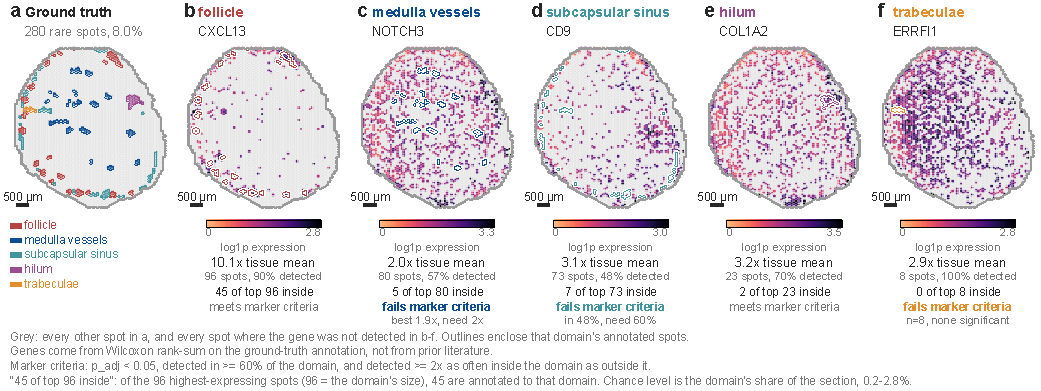
\includegraphics[width=\textwidth]{fig10_marker_fields}
\caption{Marker expression fields for the five rare domains. For each domain, the most specific gene found by full-ranking Wilcoxon screening, plotted on the tissue. Follicle shows the only spatially specific marker (CXCL13). Hilum's COL1A2 passes the statistical criteria but is high across the whole capsule, so the field does not localize the domain. The remaining three domains have no gene satisfying all three criteria. The panels contain no model output and cannot be read as evidence that a model detects these domains; they establish only what is present in the expression data.}
\label{fig:f10}
\end{figure*}

This matters because it removes a common assumption. When rare-F1 stays at zero, the default explanation is that the model failed to exploit a signal that is present. On this dataset, that premise is confirmed for exactly one of five rare domains and unverified for the other four. Any claim that a method ``recovers rare domains'' on this section is, for four of the five domains, a claim about a signal whose presence has not been established.

\subsection{The public-code baseline that motivated the rebuild}

Figure~\ref{fig:f4} reports the paired differences under the original (public-code) basis, and it is the direct empirical motivation for the aligned-basis re-measurement in Section~\ref{sec:aligned} rather than an appendix to it. The differences sit at the $10^{-3}$ scale, flip sign across seeds, and the rare-F1 difference is zero because neither arm can produce a sub-threshold cluster under the default partition. These are not a null result about spatial relations. They are a demonstration that the comparison had no headroom, which is the problem the aligned basis was built to remove.

\begin{figure*}[tbp]
\centering
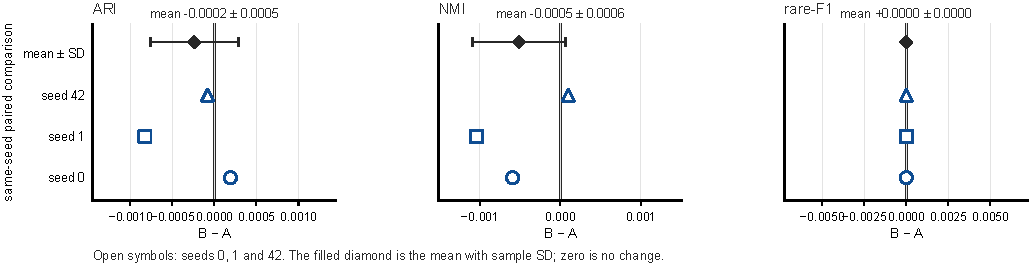
\includegraphics[width=\textwidth]{fig4_paired_metrics}
\caption{Paired differences under the public-code baseline, the comparison that motivated the rebuild. Same-seed B $-$ A differences for ARI, NMI, and rare-F1, with individual seeds as open circles and the mean $\pm$ s.d. as a filled diamond. The differences sit at the $10^{-3}$ scale and flip sign across seeds, and the rare-F1 difference is zero because neither arm can produce a sub-threshold cluster under this partition. This is the empirical signature of a comparison with no headroom.}
\label{fig:f4}
\end{figure*}

Two further figures document the rare-spot routing under these arms. Figure~\ref{fig:f3} traces where rare spots are assigned, and Figure~\ref{fig:f2} shows the per-arm partitions against the ground truth.

\begin{figure*}[tbp]
\centering
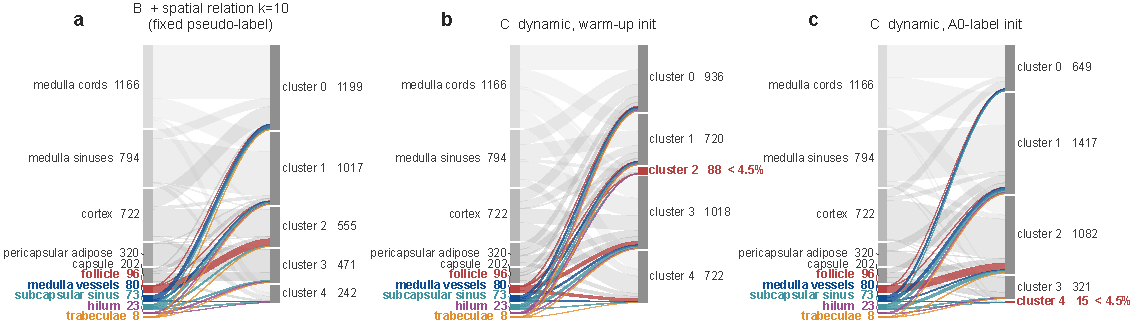
\includegraphics[width=\textwidth]{fig3_rare_flow}
\caption{Where rare spots go. Rare-domain flow from their true annotation to the clusters they are assigned to. Ribbon width is the number of spots; red cluster bars mark clusters below the 4.5\% threshold. The figure describes which spots were grouped together and cannot by itself rule out a spatial effect or establish that cluster-slot allocation is the sole cause.}
\label{fig:f3}
\end{figure*}

\section{Discussion}
\label{sec:discussion}

\subsection{What generalizes}

Two of our findings are about methodology and should transfer beyond this dataset.

The first is the headroom calculation of Section~\ref{sec:headroom}. Before comparing two architectural variants, measure how far the model can deviate from its starting point, and treat that number as the resolution limit of the comparison. A pipeline whose output is pinned by a frozen target cannot evaluate architecture in that regime, and reporting the resulting null as evidence about the architecture is an error of interpretation rather than a shortage of compute. The diagnostic is a Hungarian alignment and a count; it costs seconds and it can invalidate an entire experimental design.

The second is the construction argument of Section~\ref{sec:construction}. A rare-domain F1 of zero is only informative when paired with the partition's own attainable F1. When the initial partition contains no small cluster, the endpoint is pinned by construction and the null carries no information about the model. This too is cheap to check and does not require ground truth---only the partition and the rarity threshold.

We would add a third, smaller observation that cost us a round of experiments: an architectural component must be checked for whether it is actually active under the batching scheme before it is compared. A relation that survives in the graph but never co-occurs within a batch cannot be evaluated.

\subsection{What is specific}

The magnitude and even the sign of the spatial-relation effect depend on the graph construction, the batching scheme, and the partition. Our negative result in Section~\ref{sec:aligned} applies to an unweighted kNN graph under matched sampling, on one section. The literature's positive spatial results typically weight or refine the graph, and nothing here rules that out; Section~\ref{sec:aligned} is evidence that uniform spatial adjacency alone is insufficient, which is a narrower claim than the field's framing sometimes invites.

The prototype-clustering result is likewise scoped. The failure we observe is the interaction of a weak warm-up representation with an iteratively updated clustering objective. If the warm-up representation carried domain structure, the same prototype update might behave differently. Our result does not say prototype clustering is unworkable; it says it did not work when initialized from a representation whose kNN purity was 1.3 percentage points above chance.

\subsection{Limitations}

The scope of these results is bounded in ways worth stating plainly. All experiments use one human lymph node section and RNA alone; the ADT modality present in the source data went unused, and a second spatial dataset was under consideration when the project stopped, so no cross-dataset generalization is claimed. The section carries 3{,}484 spots and the rarest domain only 8, so per-domain recall estimates are dominated by small counts and that 8-spot domain cannot support any strong claim. The primary endpoint uses a 4.5\% cutoff; the closest alternative convention ($\leq 5\%$) changes exactly one run's value in our set, but we did not sweep the threshold systematically. The aligned-basis comparison in Section~\ref{sec:aligned} reports 30-epoch warm-up metrics rather than full 100-epoch runs, which isolates the representation effect at the cost of comparability between its absolute numbers and those reported elsewhere here. Because the project stopped under a pre-registered gate, the full four-arm ablation, the $\tau/\delta$ calibration, and graph refinement were never run, and we make no claims about them. Finally, the domain labels are an annotation layer rather than biology: disagreement between a method and these labels is not the same as a method error, particularly at the boundaries that define the rare domains.

\subsection{A note on reporting negative results}

We are reporting a stopped project whose central comparisons are null or negative. The methodological finding is the transferable part: the specific numbers are bound to this dataset, but the headroom diagnostic and the construction argument are not. The artifacts required to falsify our conclusions are also preserved. A reader who suspects that our negative result reflects an implementation error has everything needed to check, including the null controls (coordinate-shuffled and degree-preserving rewirings, relation-off freezing) and the wiring evidence that the spatial relation was live. We would rather publish a well-instrumented negative than an unverifiable positive. Negative results in this area are under-reported, and their absence distorts the literature: when only positive outcomes are written up, the apparent success rate of architectural modifications is inflated, and the diagnostics that explain why a modification fails are lost. Those diagnostics are often the most useful thing a project produces. Publishing this costs us a favourable-looking result we do not have; not publishing it would cost the field a measurement it needs.

\section{Conclusion}
\label{sec:conclusion}

The question we set out to answer was whether a frozen pseudo-label is what keeps a spatial transcriptomics model from recovering rare tissue domains. The answer, on one human lymph node section, is that the lock is real but it is not the limit. The model trained against the frozen label reproduces it, changing 0 of 3{,}484 assignments at one seed, so the comparison that was supposed to test spatial relations and dynamic clustering measured noise instead. Releasing the lock does not rescue the outcome. On a basis where the output could move freely, the unweighted spatial relation reduced structural agreement on all three seeds, and the prototype mechanism meant to correct the initial partition erased the small cluster it was handed. Neither remedy recovered the rare domains.

What the failure leaves behind are two diagnostics that travel. A rare-domain F1 of zero under a 5-way partition is not a cluster-count ceiling, since the attainable value over merges of the annotation is 1.0000; the endpoint is pinned by whether the initial partition happens to contain a cluster below the rarity threshold, which is a property of the partition, not of the model. And a null measured under a frozen target is guaranteed by the design rather than discovered from the data, a hazard that applies wherever an architecture is compared against a target it has already learned to reproduce. Applied before the comparison, both would have told us that the first round of experiments could not answer the question they were built to answer.

Both diagnostics are cheap to compute and should precede the comparison they validate. Applied earlier, they would have redirected this project before its first training run.

\section{Reproducibility and artifacts}
\label{sec:repro}

All numbers in this report are read programmatically from run outputs rather than transcribed by hand; each figure cites the run directory and protocol hash it derives from. The aligned-basis comparison (Section~\ref{sec:aligned}) is backed by a strict paired report and per-seed run directories, with coordinate-shuffled, degree-preserving-rewiring, and relation-off null controls; the rewiring control is the load-bearing one, since it fixes the degree sequence and randomizes the topology, so its parity with the true graph isolates topology as the thing that failed to help. The frozen-target headroom (Section~\ref{sec:headroom}) rests on Hungarian-aligned per-spot change counts for both arms across three seeds. The construction proof (Section~\ref{sec:construction}) is an exhaustive enumeration over all 42{,}525 5-way merges of the 10 annotated domains. Batching retention (Section~\ref{sec:batching}) was measured under uniform, bisected, and bisected-plus-halo sampling. The warm-up representation (Section~\ref{sec:prototype}) was probed at 20-epoch intervals through 100 epochs. The marker analysis (Section~\ref{sec:markers}) reports per-domain Wilcoxon statistics with the stated thresholds and a threshold-robustness check.

The upstream method this work builds on is scFormer; its released code is used unmodified as the baseline. Code and configuration for the work reported here are released under the MIT license. All runs carry a protocol SHA-256 recorded in their output directories, so a reported result can be traced to the exact configuration that produced it.

\paragraph{Figures.} Fig.~\ref{fig:f1}: ground-truth domains and the five rare domains. Fig.~\ref{fig:f2}: per-arm spatial partitions. Fig.~\ref{fig:f3}: rare-domain flow. Fig.~\ref{fig:f4}: paired differences under the public-code baseline. Fig.~\ref{fig:f5}: in-batch spatial-edge retention under three batching schemes. Fig.~\ref{fig:f6}: warm-up representation structure. Fig.~\ref{fig:f7}: prototype refresh dynamics. Fig.~\ref{fig:f8}: rare-domain F1 and ARI across Leiden resolutions. Fig.~\ref{fig:f9}: method design versus ablation status. Fig.~\ref{fig:f10}: marker expression fields. Fig.~\ref{fig:f11}: initial versus final partitions for the dynamic arm. Fig.~\ref{fig:f12}: the aligned-basis result and its null controls.

Eleven of the twelve figures (\ref{fig:f1} through \ref{fig:f11}) were produced with the project's figure pipeline from the run artifacts cited above; the remaining figure (\ref{fig:f12}) was produced for this report. All are regenerable from the released code and the run outputs. Spot-level panels restore Visium array coordinates to physical geometry (100\,\textmu m column pitch, 86.6\,\textmu m row pitch) and render each spot as its Voronoi tile.

\begin{thebibliography}{99}
\bibitem{scformer} Huang, J., Xia, X., Luo, F., Qu, L., Feng, X., Zheng, L. Specificity-driven cell--gene graph learning identifies rare cell states in single-cell and spatial transcriptomic data. \emph{Advanced Biotechnology} \textbf{4}(3), 26 (2026). DOI: 10.1007/s44307-026-00121-y.
\bibitem{traag} Traag, V. A., Waltman, L., van Eck, N. J. From Louvain to Leiden: guaranteeing well-connected communities. \emph{Scientific Reports} \textbf{9}, 5233 (2019). DOI: 10.1038/s41598-019-41695-z.
\bibitem{dec} Xie, J., Girshick, R., Farhadi, A. Unsupervised deep embedding for clustering analysis. \emph{Proceedings of the 33rd International Conference on Machine Learning} (PMLR) \textbf{48}, 478--487 (2016).
\bibitem{desc} Li, X., Wang, K., Lyu, Y., Pan, H., Zhang, J., Stambolian, D., Susztak, K., Reilly, M. P., Hu, G., Li, M. Deep learning enables accurate clustering with batch effect removal in single-cell RNA-seq analysis. \emph{Nature Communications} \textbf{11}, 2338 (2020). DOI: 10.1038/s41467-020-15851-3.
\bibitem{deepdpm} Ronen, M., Finder, S. E., Freifeld, O. DeepDPM: deep clustering with an unknown number of clusters. \emph{2022 IEEE/CVF Conference on Computer Vision and Pattern Recognition (CVPR)}, 9851--9860 (2022). DOI: 10.1109/CVPR52688.2022.00963.
\bibitem{stagate} Dong, K., Zhang, S. Deciphering spatial domains from spatially resolved transcriptomics with an adaptive graph attention auto-encoder. \emph{Nature Communications} \textbf{13}, 1739 (2022). DOI: 10.1038/s41467-022-29439-6.
\bibitem{graphst} Long, Y., Ang, K. S., Li, M., Chong, K. L. K., Sethi, R., Zhong, C., Xu, H., Ong, Z., Sachaphibulkij, K., Chen, A., Zeng, L., Fu, H., Wu, M., Lim, L. H. K., Liu, L., Chen, J. Spatially informed clustering, integration, and deconvolution of spatial transcriptomics with GraphST. \emph{Nature Communications} \textbf{14}, 1155 (2023). DOI: 10.1038/s41467-023-36796-3.
\bibitem{spatialglue} Long, Y., Ang, K. S., Sethi, R., Liao, S., Heng, Y., van Olst, L., et al. Deciphering spatial domains from spatial multi-omics with SpatialGlue. \emph{Nature Methods} \textbf{21}(9), 1658--1667 (2024). DOI: 10.1038/s41592-024-02316-4.
\bibitem{spamics} Cai, G., Chen, F., Wen, K., Li, Y., Ou-Yang, L. Identifying spatial domains from spatial multi-omics data using consistent and specific deep subspace learning. \emph{Information Fusion} \textbf{125}, 103428 (2026). DOI: 10.1016/j.inffus.2025.103428.
\bibitem{stkeep} Zuo, C., Xia, J., Chen, L. Dissecting tumor microenvironment from spatially resolved transcriptomics data by heterogeneous graph learning. \emph{Nature Communications} \textbf{15}, 5057 (2024). DOI: 10.1038/s41467-024-49171-7.
\bibitem{stahl} St{\aa}hl, P. L., Salm{\'e}n, F., Vickovic, S., Lundmark, A., Fern{\'a}ndez Navarro, J., Magnusson, J., et al. Visualization and analysis of gene expression in tissue sections by spatial transcriptomics. \emph{Science} \textbf{353}(6294), 78--82 (2016). DOI: 10.1126/science.aaf2403.
\bibitem{rao} Rao, A., Barkley, D., Fran{\c c}a, G. S., Yanai, I. Exploring tissue architecture using spatial transcriptomics. \emph{Nature} \textbf{596}(7871), 211--220 (2021). DOI: 10.1038/s41586-021-03634-9.
\bibitem{hubert} Hubert, L., Arabie, P. Comparing partitions. \emph{Journal of Classification} \textbf{2}(1), 193--218 (1985). DOI: 10.1007/BF01908075.
\bibitem{sklearn} Pedregosa, F., Varoquaux, G., Gramfort, A., Michel, V., Thirion, B., Grisel, O., et al. Scikit-learn: machine learning in Python. \emph{Journal of Machine Learning Research} \textbf{12}(85), 2825--2830 (2011).
\end{thebibliography}

\end{document}
